% !TeX root = ../index.tex

\section{Hardwareschicht}
\textit{TODO Kevin Hoss: Noch in Bearbeitung}

Wie bereits im vorherigen Kapitel angedeutet bildet die Hardwareschicht den untersten Baustein der Systemarchitektur. In diesem Kapitel werden die Methoden vorgestellt, die während des Laborprojekts eingesetzt wurden, um mit der Hardware arbeiten zu können. Desweiteren werden die einzelnen Hardwarebestandteile aufgedrosselt und deren Funktionsweise näher beschrieben.

Beim Arbeiten mit der eingesetzten Hardware haben wir auf die browserbasierte Anwendung Wokwi gesetzt, welche unter der URL https://wokwi.com erreichbar ist. Die Entscheidung für die virtuelle Umgebung Wokwi wurde aus dem Grund getroffen, da das Aufbauen einer Netzwerkumgebung im Labor nicht möglich war. Die Simulation in Wokwi kann allerdings im Anschluss auf die reale Welt übertragen werden und der entwickelte Code läuft auf den entsprechenden Hardwaregeräten ohne eine notwendige Konvertierung.

Bezüglich der eingesetzten Hardware kommen bei unserer intelligenten Gartenbewässerung insgesamt zwei ESP32-Mikrokontroller des Unternehmens Espressif Systems zum Einsatz. Mithilfe der Microcontroller können die angeschlossenen Sensoren und Aktoren angesteuert werden. Dabei wird ein ESP32-Mikrokontroller für die Sensoren und einer für die Aktoren eingesetzt. Im folgenden werden vorerst die Sensoren und anschließend die Aktoren näher beleuchtet.

\subsection{Hardware für Sensoren}
Als Temperatur- und Feuchtigkeitssensor setzen wir in der virtuellen Wokwi Umgebung auf einen DHT22 Sensor. Insgesamt setzen wir davon zwei Stück ein, einen für die Werte in der Luft und einen für die Werte im Boden. In der realen Welt kann der DHT22 Sensor allerdings nicht im Erdboden vergraben werden, da dieser nicht wasserresistent ist. In der Wokwi Umgebung gibt es allerdings nur eine begrenzte Auswahl an Hardwaresensorik. Im realen Anwendungsfall würde sich ein \textit{-muss ich noch rausfinden-} Sensor für die Ermittlung der Temperatur- und Feuchtigkeitswerte eignen. In Wokwi steht der zweite DHT22 Sensor somit repräsentativ für die Temperatur- und Feuchtigkeitswerte im Boden.

\textit{Hier kommt noch Text zu Sensoren}

In Abb. \ref{fig:wokwi_sensoren} ist ein visueller Auszug aus Wokwi dargestellt, welcher den Anschluss der Sensorik an den ESP32-Mikrokontroller beinhaltet.

\begin{figure}[h]
    \centering
    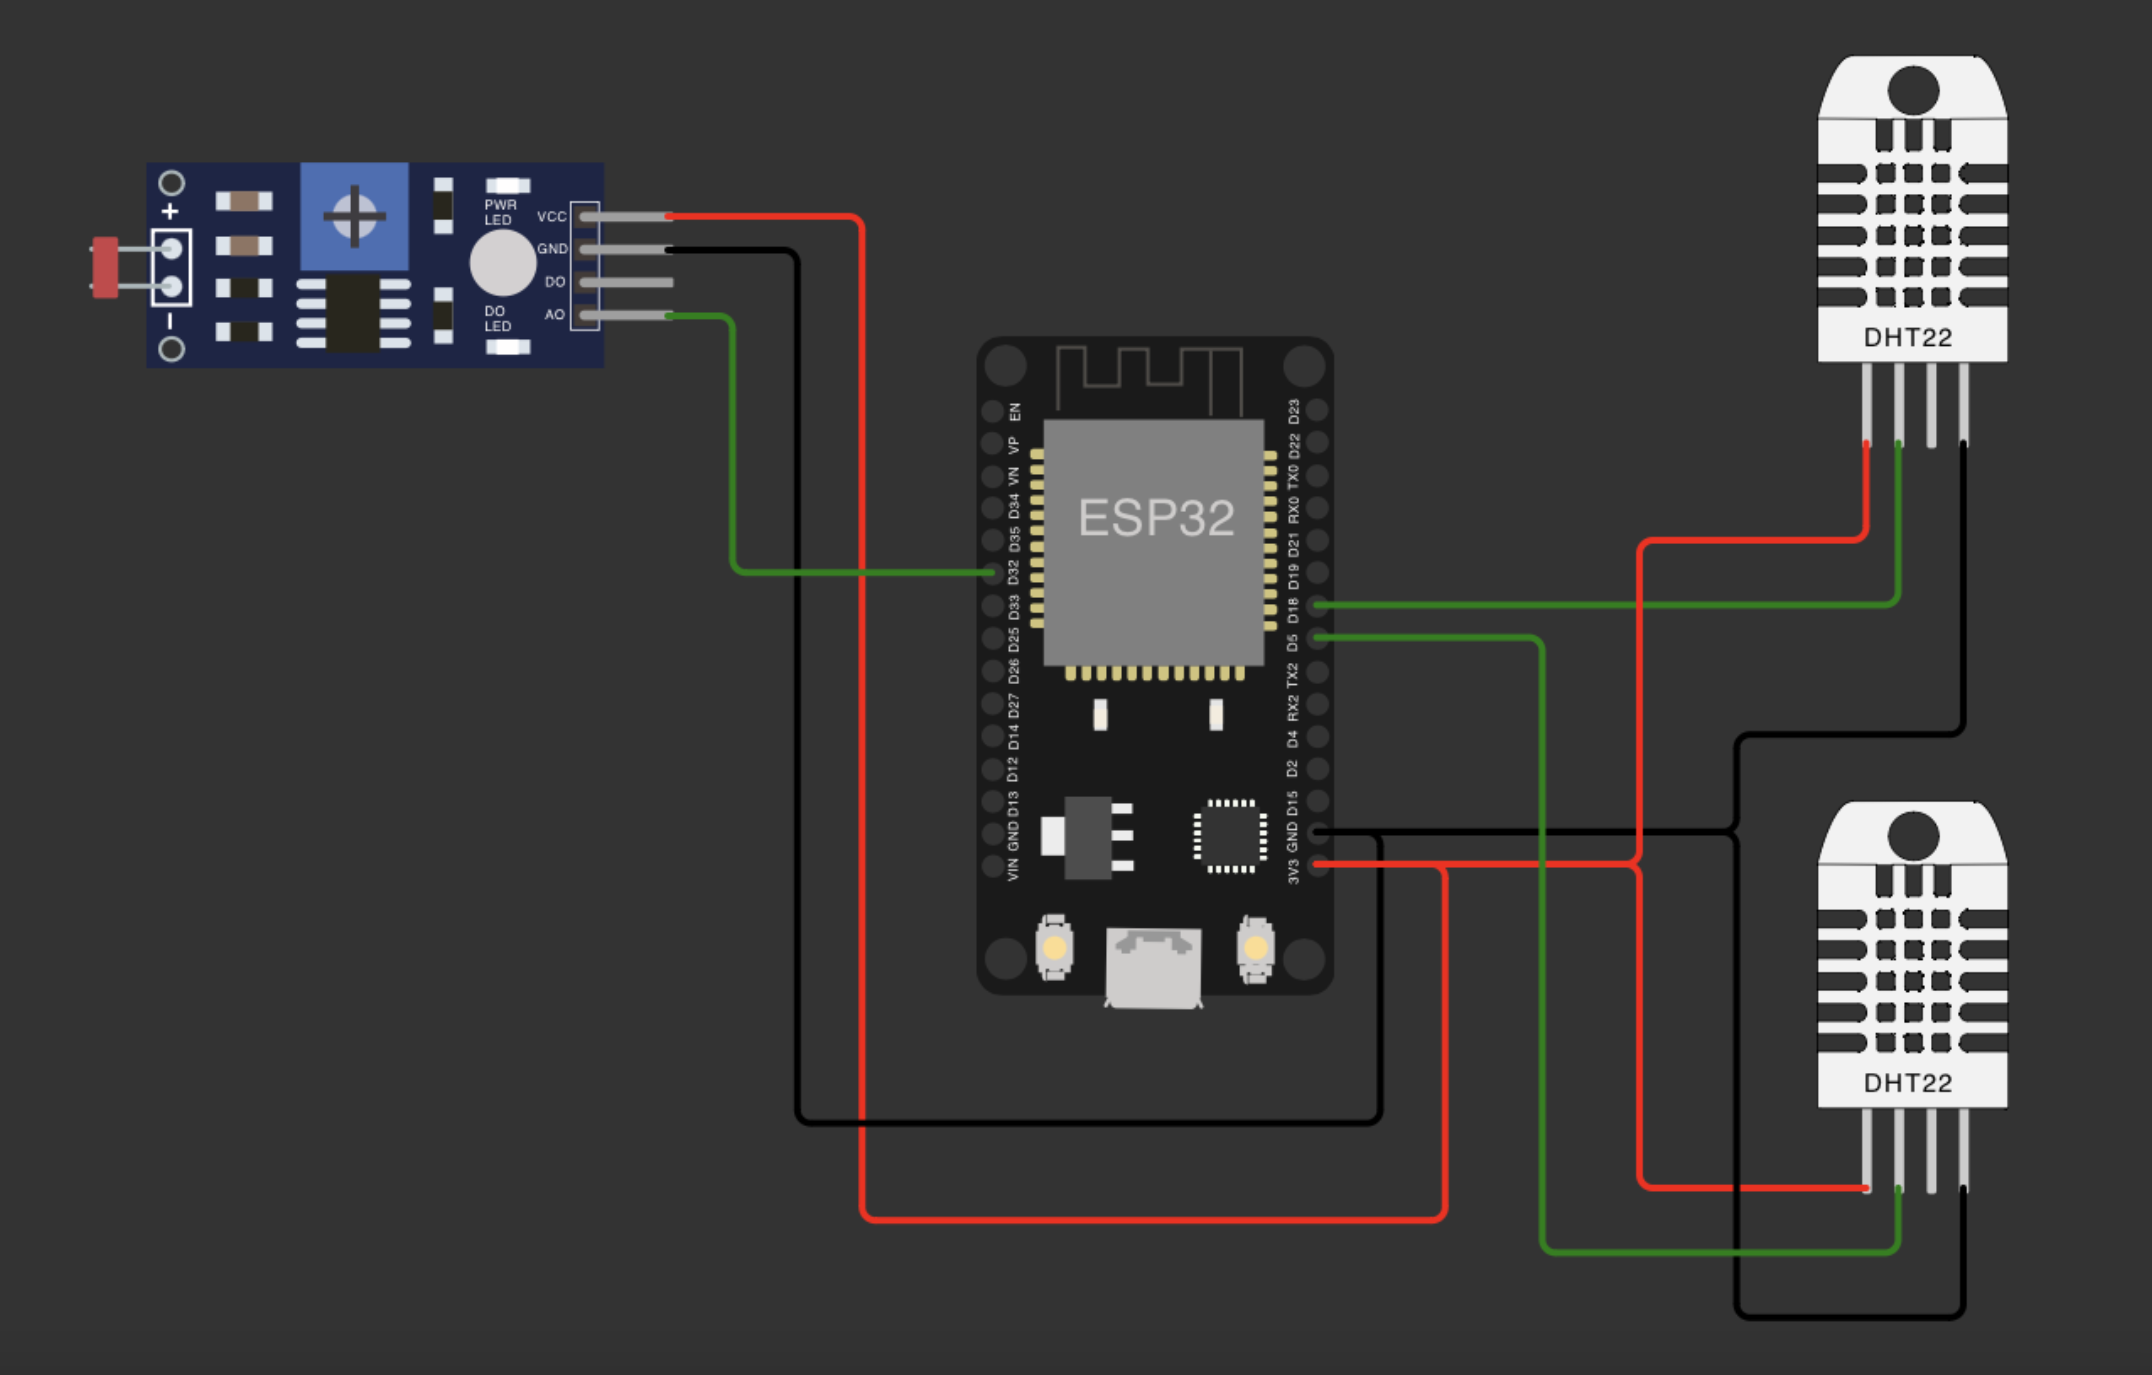
\includegraphics[width=0.8\textwidth]{Wokwi_Sensoren.png}
    \caption{Anschluss der Sensorhardware in der virtuellen Umgebung Wokwi}\label{fig:wokwi_sensoren}
\end{figure}

\subsection{Hardware für Aktoren}
\textit{Hier kommt Text zu Aktoren}

\begin{figure}[h]
    \centering
    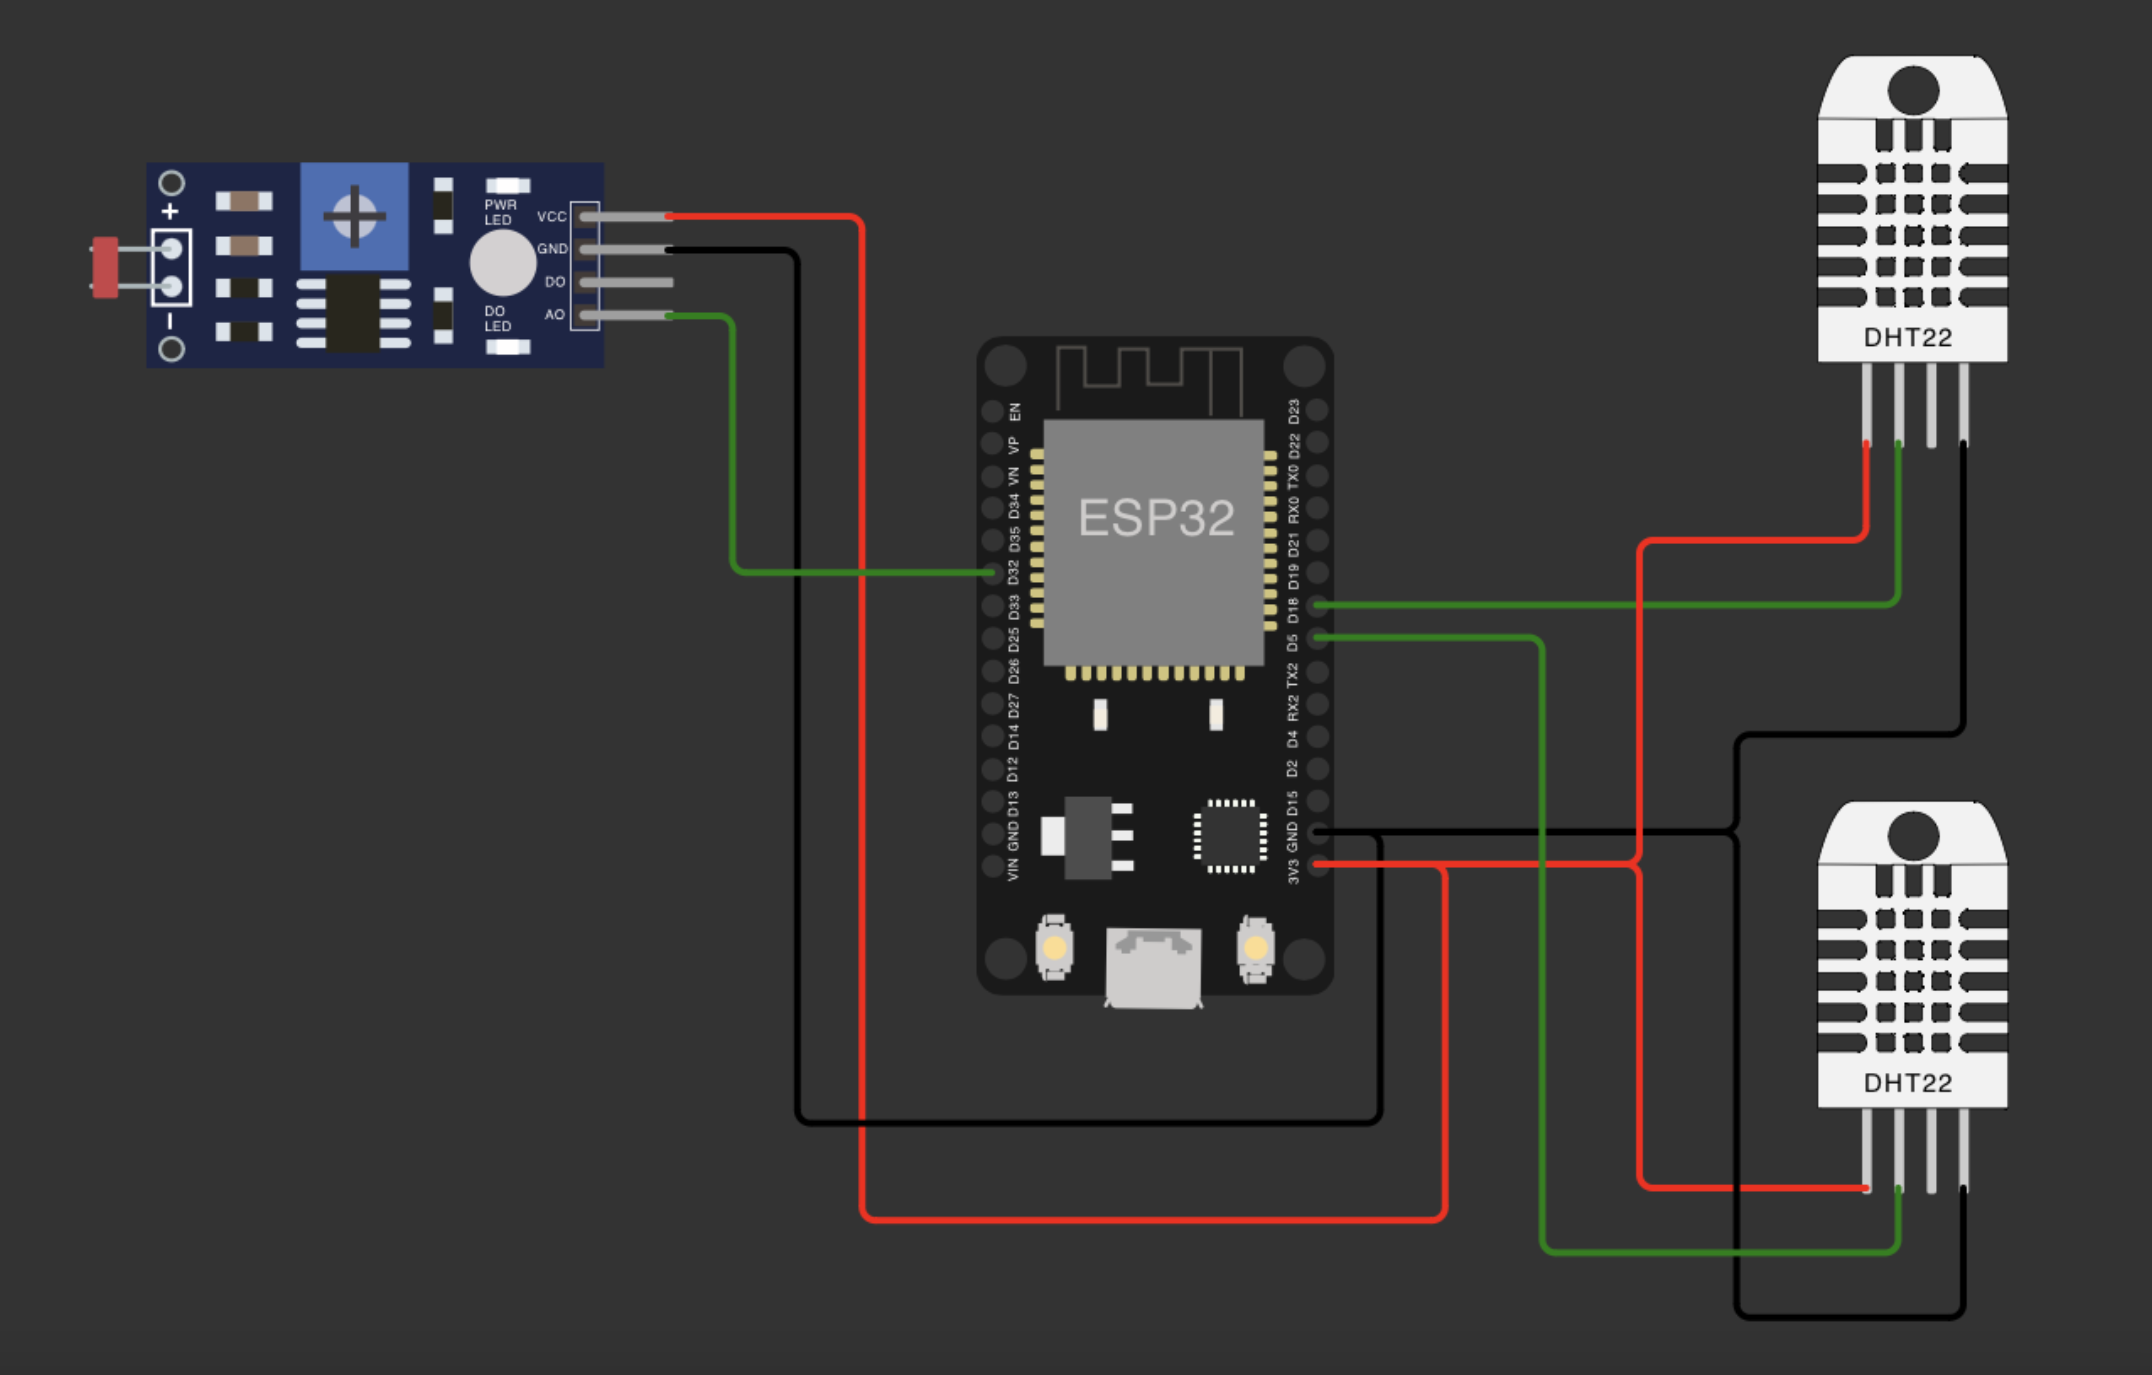
\includegraphics[width=0.8\textwidth]{Wokwi_Sensoren.png}
    \caption{Anschluss der Aktorenhardware in der virtuellen Umgebung Wokwi}\label{fig:wokwi_aktoren}
\end{figure}